% Floats are issued here, one page before they are discussed, so they can land on pages 2 and 3. Fig. 2 comes before
% Fig. 3 in the source so that the figures are numbered in order.
% Generated by python -m src.seeds_tables; needs \usepackage{booktabs}.
\begin{table*}[t]
\centering
\small
\setlength{\tabcolsep}{3pt}
\caption{Every perceptual loss costs PSNR against L1; the best LPIPS and DISTS values lie within one seed spread of each other, and statistics matching gives DINOv2-S its best texture. Test split (220 slices, 31 patients, 100k). Values: mean$\pm$std over seeds 42, 123 and 456. Bold: best trained configuration. $^{\dagger}$ significantly better and $^{\ddagger}$ significantly worse than C0 (L1) (paired Wilcoxon on seed-averaged slices, Holm over 30 tests, p < 0.05; PSNR, LPIPS and $|1-R_H|$ only). * scored with its own training metric. point.: pointwise, stat.: local statistics matching.}
\label{tab:results}
\begin{tabular}{lllcccccc}
\toprule
ID & Network & Matching & PSNR (dB) $\uparrow$ & SSIM $\uparrow$ & LPIPS $\downarrow$ & DISTS $\downarrow$ & $R_H$ ($\to$1) & $|1-R_H|$ $\downarrow$ \\
\midrule
 & LDCT input &  & 23.04 & 0.7423 & 0.2843 & 0.1641 & 6.174 & 5.275 \\
C0 & -- & -- & \textbf{30.92$\pm$0.07} & \textbf{0.8691$\pm$0.0025} & 0.1043$\pm$0.0010 & 0.1112$\pm$0.0006 & 0.657$\pm$0.026 & 0.352$\pm$0.026 \\
C1 & VGG-19 & point. & 30.32$\pm$0.22$^{\ddagger}$ & 0.8606$\pm$0.0022 & 0.0592$\pm$0.0010$^{\dagger}$ & 0.0668$\pm$0.0023 & 0.798$\pm$0.035 & 0.226$\pm$0.030$^{\dagger}$ \\
C2 & LPIPS-VGG & point. & 30.39$\pm$0.31$^{\ddagger}$ & 0.8630$\pm$0.0021 & 0.0563$\pm$0.0045$^{\dagger}${}$^{*}$ & \textbf{0.0645$\pm$0.0024} & 0.777$\pm$0.012 & 0.242$\pm$0.009$^{\dagger}$ \\
C3 & DISTS & stat. & 29.81$\pm$0.20$^{\ddagger}$ & 0.8326$\pm$0.0244 & \textbf{0.0557$\pm$0.0066}$^{\dagger}$ & 0.0664$\pm$0.0014$^{*}$ & 0.820$\pm$0.014 & 0.222$\pm$0.018$^{\dagger}$ \\
C4 & RadImageNet & point. & 28.70$\pm$0.32$^{\ddagger}$ & 0.8259$\pm$0.0075 & 0.0868$\pm$0.0055 & 0.0847$\pm$0.0009 & 0.798$\pm$0.040 & 0.286$\pm$0.017$^{\dagger}$ \\
C5 & DINOv2-S & point. & 30.10$\pm$0.51$^{\ddagger}$ & 0.8625$\pm$0.0063 & 0.0629$\pm$0.0078$^{\dagger}$ & 0.0707$\pm$0.0068 & 0.682$\pm$0.046 & 0.333$\pm$0.044$^{\dagger}$ \\
C6 & DINOv2-B & point. & 30.20$\pm$0.44$^{\ddagger}$ & 0.8618$\pm$0.0044 & 0.0614$\pm$0.0027$^{\dagger}$ & 0.0713$\pm$0.0028 & 0.731$\pm$0.027 & 0.291$\pm$0.029$^{\dagger}$ \\
C7 & MedSigLIP & point. & 29.84$\pm$0.39$^{\ddagger}$ & 0.8596$\pm$0.0061 & 0.0750$\pm$0.0114$^{\dagger}$ & 0.0737$\pm$0.0070 & 0.531$\pm$0.063 & 0.477$\pm$0.060$^{\ddagger}$ \\
C8 & DINOv2-S & stat. & 30.26$\pm$0.28$^{\ddagger}$ & 0.8614$\pm$0.0068 & 0.0579$\pm$0.0112$^{\dagger}$ & 0.0654$\pm$0.0047 & 0.857$\pm$0.017 & 0.195$\pm$0.013$^{\dagger}$ \\
C9 & CT dose net v2 & point. & 30.44$\pm$0.10$^{\ddagger}$ & 0.8514$\pm$0.0219 & 0.0673$\pm$0.0031$^{\dagger}$ & 0.0973$\pm$0.0002 & 0.850$\pm$0.018 & 0.203$\pm$0.010$^{\dagger}$ \\
C10 & CT dose net v2 & stat. & 29.80$\pm$0.19$^{\ddagger}$ & 0.8475$\pm$0.0039 & 0.0721$\pm$0.0063$^{\dagger}$ & 0.0982$\pm$0.0036 & 0.951$\pm$0.058 & \textbf{0.167$\pm$0.026}$^{\dagger}$ \\
\bottomrule
\end{tabular}
\end{table*}


\begin{figure}[t]
  \centering
  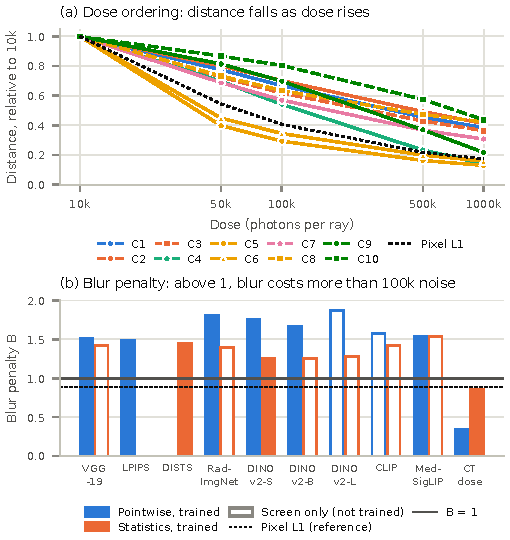
\includegraphics[width=\linewidth]{figures/fig2_screen_column}
  \caption{Training-free screen (validation split). Every pretrained network orders doses almost perfectly (a); only
    the CT dose network penalizes blur less than noise of the same pixel error (b).}
  \label{fig:screen}
\end{figure}

\begin{figure*}[t]
  \centering
  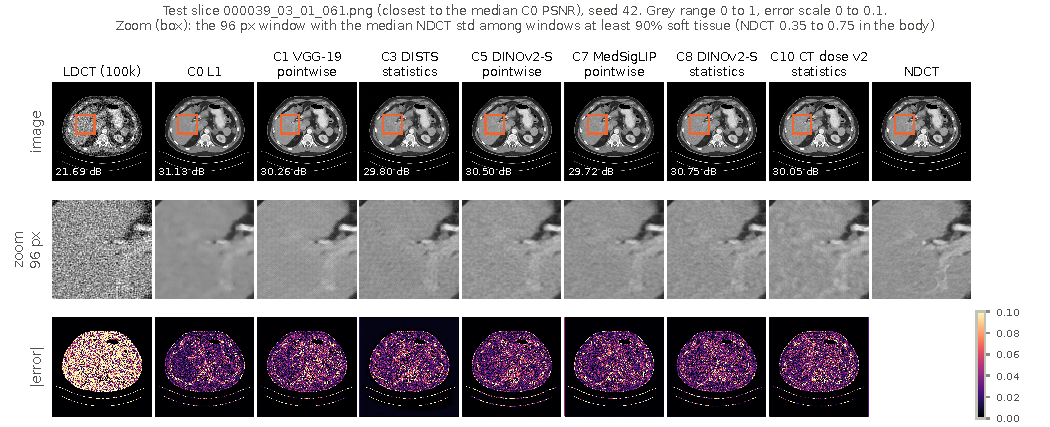
\includegraphics[width=\textwidth]{figures/fig3_qualitative}
  \caption{Test slice closest to the median C0 PSNR, seed 42. Rows: image, zoom, $\lvert \hat{x} - x \rvert$; grey
    range $[0, 1]$, error scale 0 to 0.1. Zoom: the $96 \times 96$ window with the median NDCT standard deviation
    among windows that are at least 90\% soft tissue (NDCT 0.35 to 0.75 inside the body mask). L1 smooths the grain
    away; statistics matching keeps DINOv2-S grain closer to NDCT than pointwise matching does.}
  \label{fig:qualitative}
\end{figure*}

\section{Method}
\label{sec:method}

\textbf{Objective.} A U-Net $f_\theta$ maps a low-dose slice to $\hat{x}$ and is trained against the normal-dose slice
$x$ with
\begin{equation*}
  \mathcal{L}_\phi = \lVert \hat{x} - x \rVert_1 + \lambda_\phi \, d_\phi\big(\mathrm{crop}(\hat{x}), \mathrm{crop}(x)\big),
\end{equation*}
where $\mathrm{crop}$ is one random $224 \times 224$ crop shared by prediction and target and $d_\phi$ a distance in
the features of a frozen network $\phi$. With $\bar{\phi}_l$ the channel-normalized features of
block $l$ ($C_l$ channels, $H_l \times W_l$ positions), pointwise matching is
\begin{equation}
  d^{\mathrm{pt}}_\phi(\hat{x}, x) = \sum_{l} \frac{1}{H_l W_l} \sum_{h, w}
  \big\lVert \bar{\phi}_l(\hat{x})_{hw} - \bar{\phi}_l(x)_{hw} \big\rVert_2^2 .
  \label{eq:pointwise}
\end{equation}
CT noise is random, so the output cannot copy the reference grain pixel by pixel. Local statistics matching asks
only that each $4 \times 4$ window $\omega \in \Omega_l$ of each channel has the same feature mean $\mu$ and standard
deviation $\sigma$:
\begin{equation}
  d^{\mathrm{st}}_\phi(\hat{x}, x) = \sum_{l} \frac{1}{C_l \lvert \Omega_l \rvert} \sum_{c, \omega}
  \big[ 1 - s(\hat{\mu}, \mu, c_1) \, s(\hat{\sigma}, \sigma, c_2) \big],
  \label{eq:statistics}
\end{equation}
with $s(a, b, c) = (2ab + c) / (a^2 + b^2 + c)$ and $c_1 = c_2 = 10^{-6}$: the texture term of
DISTS~\cite{ding2020dists}, applied to any network.

\textbf{Feature networks} (Table~\ref{tab:networks}): VGG-19 at relu3\_2~\cite{simonyan2015vgg};
LPIPS-VGG~\cite{zhang2018lpips} and DISTS with their own weights; RadImageNet ResNet-50, layers 1 to
3~\cite{mei2022radimagenet}; DINOv2-S and DINOv2-B, blocks 3, 6, 9~\cite{oquab2024dinov2}; MedSigLIP-448, layers 7, 14,
20~\cite{sellergren2025medgemma}. DINOv2-L and CLIP ViT-B/16~\cite{radford2021clip} enter the screen only. C8 and C10
use~(\ref{eq:statistics}), C1, C4 to C7 and C9 use~(\ref{eq:pointwise}).

\textbf{CT dose network.} A loss network should change its features when the noise level changes. Three
convolutional blocks (32, 64, 128 channels; 287,328 parameters) with a regression head predict the standardized $\log_{10}$ photon count of $128 \times 128$ training-split patches (normal dose fixed at 7),
trained with smooth L1 for 10 epochs (lowest validation loss kept) and frozen; its block outputs are the features. This
version replaced a six-class classifier after a validation screen; the adoption threshold on $M_\phi$ was lowered
from 0.9 to 0.8 after seeing the screen, and the runs of the first version are an ablation in the repository. Unlike SACNN~\cite{li2020sacnn}, its features
are trained on dose alone.

\textbf{Matched influence and screen.} As in~\cite{viana2025perceptual}, we set $\lambda_\phi = 19 \, S_1 / S_\phi$,
so the perceptual term is 95\% of the loss at initialization ($S_1$, $S_\phi$: summed L1 and feature terms of the untrained
U-Net). Before training, each network is screened on the 182 validation slices: the dose ordering $M_\phi$ is the mean
Spearman correlation between $d_\phi(x^{(d)}, x)$ and $\log(1/d)$ over five photon counts $d$ from $10^4$ to $10^6$,
and the blur penalty $B_\phi$ is the summed distance of a Gaussian blur divided by that of the $10^5$ noise at equal
MSE. $B_\phi < 1$ means a denoiser can lower the loss by smoothing. Every network is trained regardless of its score.

% Generated by python -m src.seeds_tables; needs \usepackage{booktabs}.
\begin{table}[t]
\centering
\small
\setlength{\tabcolsep}{3pt}
\caption{Feature networks. Every pretrained network orders doses (M ≥ 0.95); only the CT dose network has B < 1. $^{\dagger}$ feature extractor of the CT dose network v2 (three conv blocks). $\lambda$: frozen loss weight. M: dose ordering, B: blur penalty of the training-free screen.}
\label{tab:networks}
\begin{tabular}{lllrrrr}
\toprule
ID & Network & Matching & Params (M) & $\lambda$ & M $\uparrow$ & B \\
\midrule
C1 & VGG-19 & point. & 1.15 & 4.699 & 1.000 & 1.51 \\
C2 & LPIPS-VGG & point. & 14.71 & 9.162 & 0.998 & 1.48 \\
C3 & DISTS & stat. & 14.71 & 6.984 & 0.984 & 1.45 \\
C4 & RadImageNet & point. & 25.56 & 2.211 & 0.954 & 1.81 \\
C5 & DINOv2-S & point. & 22.06 & 1.634 & 0.998 & 1.75 \\
C6 & DINOv2-B & point. & 86.58 & 2.497 & 0.997 & 1.67 \\
C7 & MedSigLIP & point. & 428.57 & 3.755 & 0.999 & 1.53 \\
C8 & DINOv2-S & stat. & 22.06 & 1.966 & 0.997 & 1.26 \\
C9 & CT dose net v2 & point. & 0.29$^{\dagger}$ & 1.549 & 0.971 & 0.34 \\
C10 & CT dose net v2 & stat. & 0.29$^{\dagger}$ & 2.802 & 0.852 & 0.86 \\
\bottomrule
\end{tabular}
\end{table}

